% !TEX root = ../AnonymousSubmission2027.tex
\section{Related Work}
\label{sec:related}

\begin{figure*}[t]
    \centering
    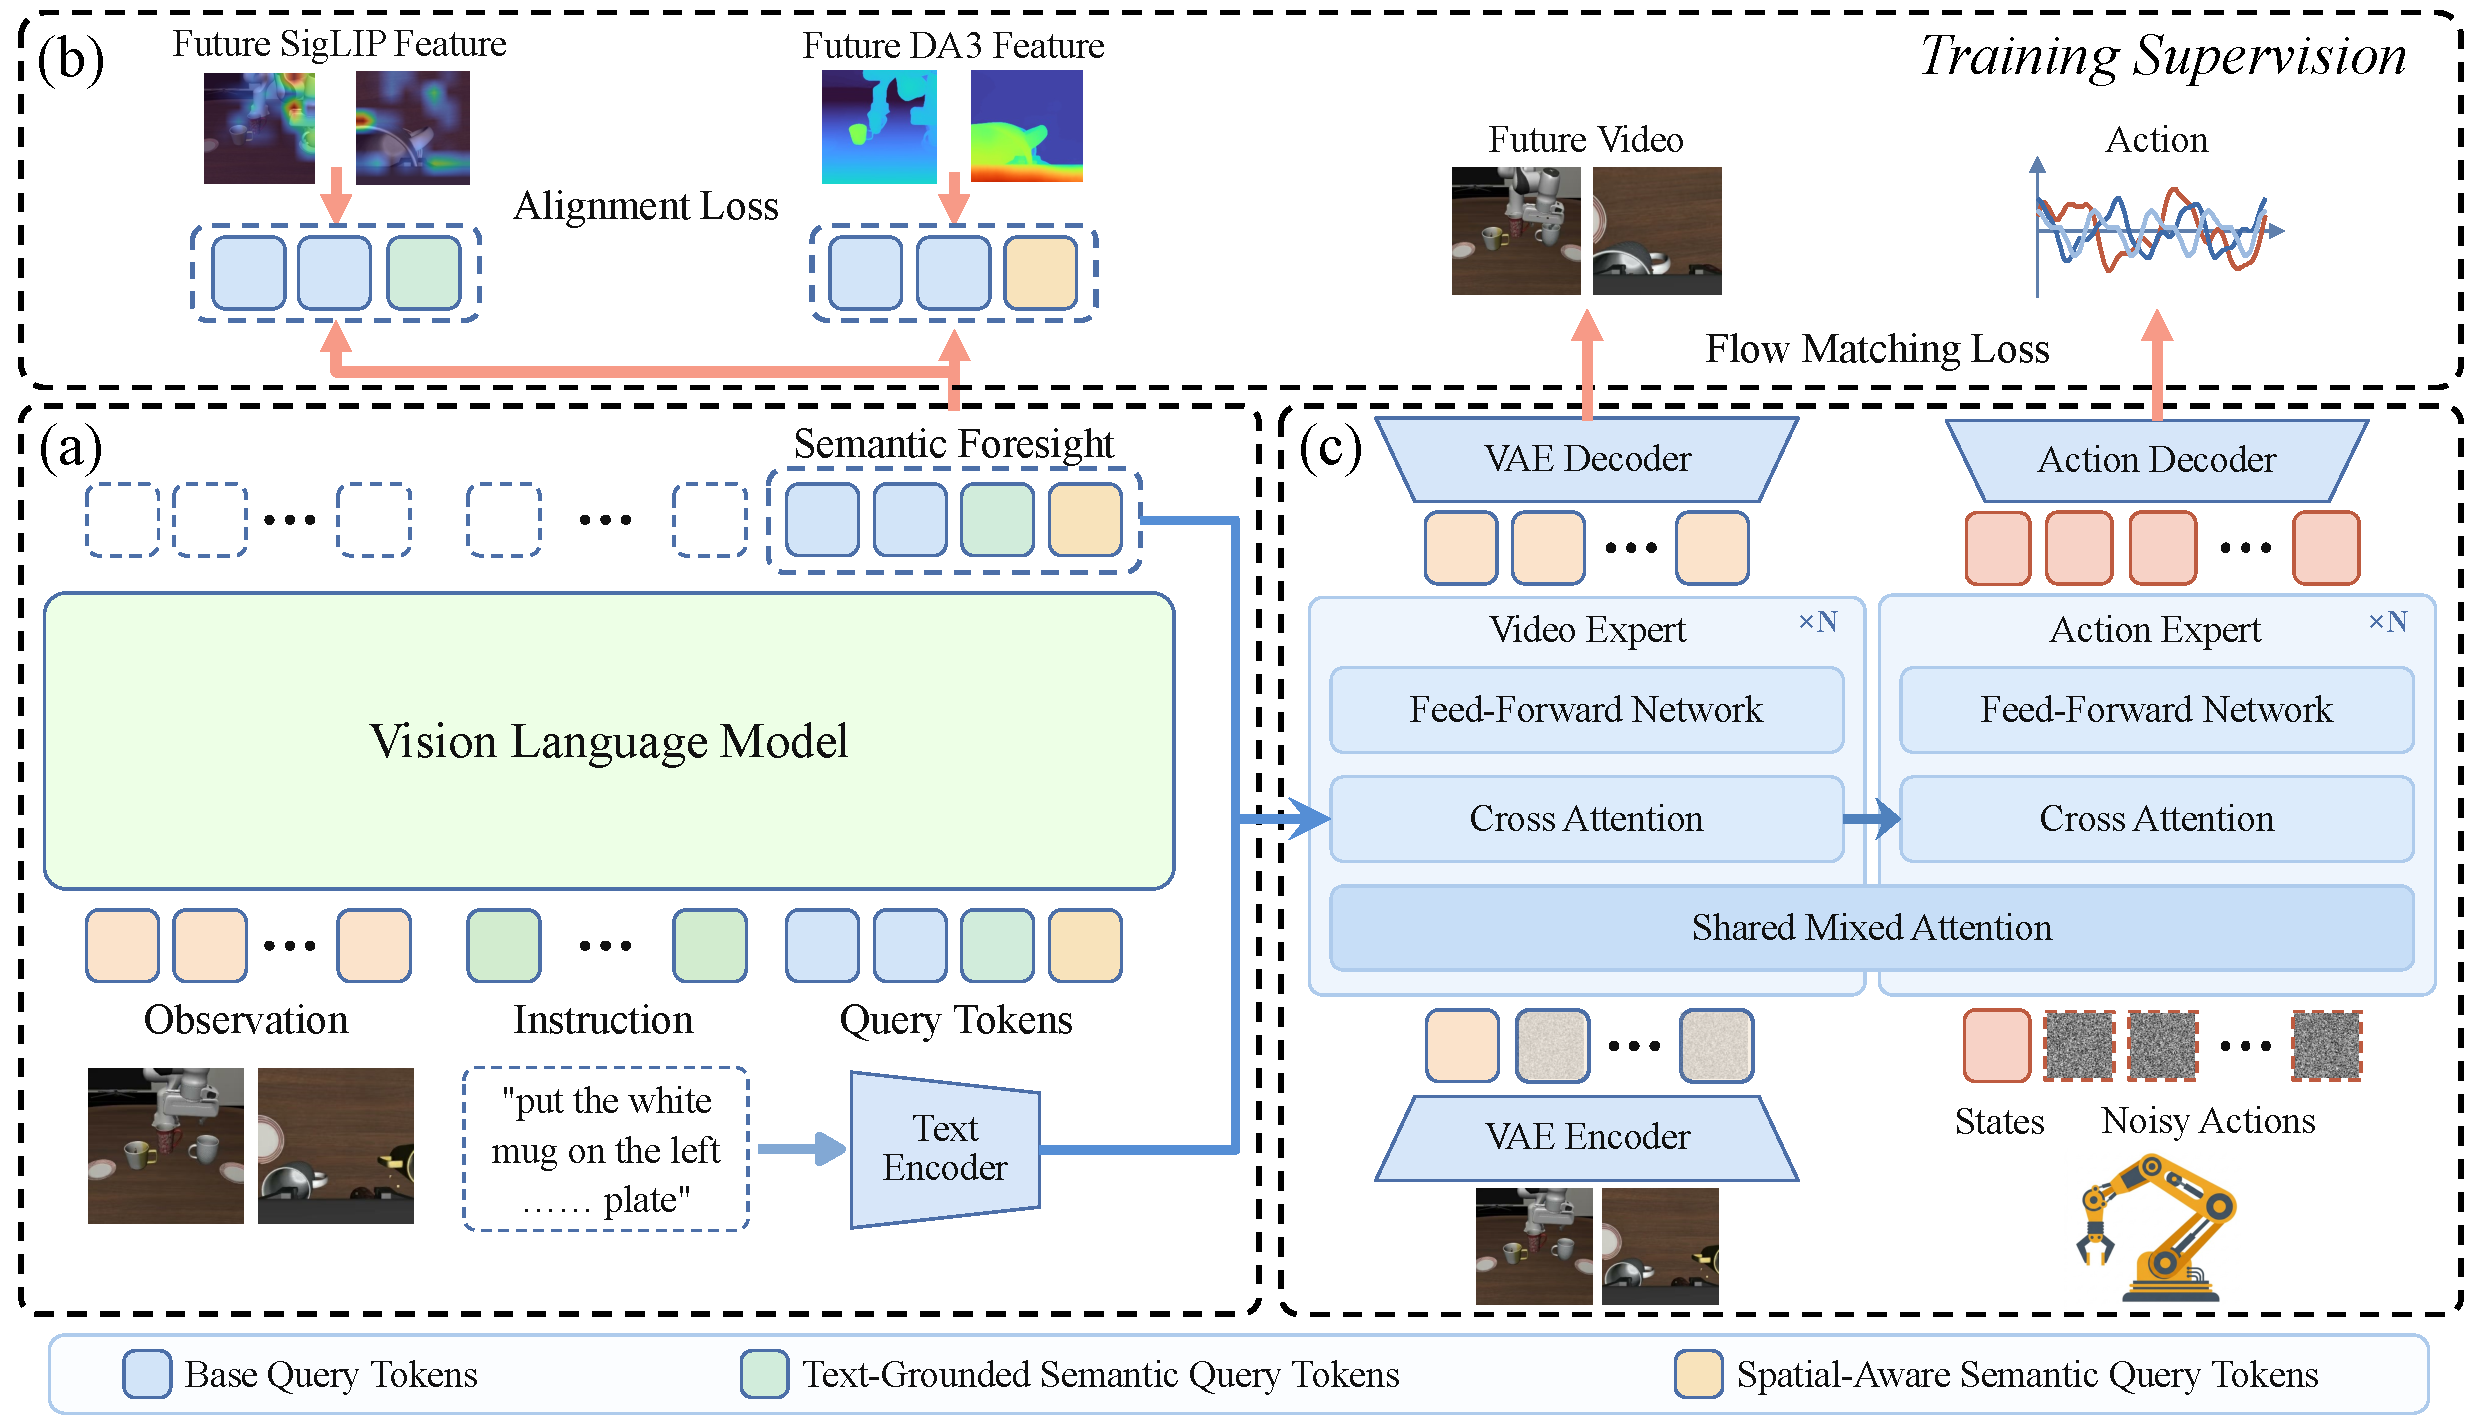
\includegraphics[width=\textwidth]{Figures/model_arch.pdf}
    \caption{\textbf{Overview of our \ourmethod.} (a) From the current observation and the language instruction, the vision-language model (VLM) planner reads out text-grounded and spatial-aware semantic foresight from a base query group and two modality-specific query groups. (b) During training, the predicted foresight is aligned with the SigLIP2 and Depth Anything~3 features of the future keyframes, while the generated video and actions are supervised by a flow-matching loss. (c) Conditioned on this semantic guidance, the world-action model generates the future frames and the action chunk through a video expert and an action expert coupled by joint attention. \rev{The foresight is predicted for each future keyframe $k$ and camera view $v$ (Eqs.~\eqref{eq:resampler}--\eqref{eq:planner_loss}), and it enters the video expert through an additional cross-attention branch that runs in parallel with the retained cross-attention to the original text-encoder embeddings of the instruction.}}
% TODO(figure): redraw Fig. 2 with keyframe/view indices on the foresight maps and a separate arrow for the retained text-encoder path (R3 suggestion).
    \label{fig:overview}
\end{figure*}

\paragraph{World-Action Models for Embodied Control}
World-action models leverage the generative priors of video backbones to predict how the scene evolves under interaction.
Early attempts generate instruction-conditioned videos and recover actions from them~\cite{unipi}, pretrain policies with video generation objectives~\cite{gr1,gr2,rynnvla}, or condition actions on the predictive representations of video diffusion models~\cite{vpp}.
More recent systems couple video foundation models with action experts at scale: Genie Envisioner~\cite{genieenvisioner} attaches a flow-matching action decoder to an instruction-conditioned video diffusion backbone, Cosmos Policy~\cite{cosmospolicy} directly fine-tunes a pretrained video model into a policy, LingBot-VA~\cite{lingbotva} interleaves video and action tokens for causal video-action world modeling, and a family of unified architectures jointly models the two modalities within a single transformer~\cite{uwm,uva,worldvla,dit4dit,fastwam}.
However, across these designs, the instruction enters generation only as coarse text embeddings~\cite{radford2021learning,raffel2020exploring} or plain text tokens, and the predicted futures capture physical dynamics rather than instruction semantics, so the generation easily drifts away from the task.

\paragraph{Guidance for Robot Manipulation}
Beyond plain text conditioning, many efforts supply manipulation models with intermediate guidance.
One line predicts visual subgoals: CoT-VLA~\cite{zhao2025cot} generates subgoal images as a visual chain of thought before decoding actions, and DreamVLA~\cite{zhangdreamvla} forecasts world knowledge such as dynamic regions and depth ahead of acting.
\rev{Closest to our feature-space foresight, LaDi-WM~\cite{ladiwm} learns a latent diffusion world model over DINO geometric and CLIP-family semantic features and lets a diffusion policy refine its actions on the imagined future latents, while DreamVLA predicts dynamic, depth, and semantic knowledge with the VLA's own tokens and decodes actions from them without generating future frames.
\ourmethod differs from both in where the foresight is predicted and how it is used: a VLM reads the observation and the instruction once and predicts future SigLIP2 and Depth Anything~3 features through learnable query tokens in a single forward pass, instead of rolling out a separate latent world model, and the prediction is injected as guidance into every block of a pretrained video-generation backbone, so that it steers future-video generation and, through joint attention, action decoding, rather than serving as an input feature of the policy.}
Within world-action models, MaskWAM~\cite{maskwam} takes first-frame masks as visual prompts and predicts future masks alongside RGB frames, Mask World Model~\cite{maskwm} forecasts the evolution of semantic masks instead of pixels, and OA-WAM~\cite{oawam} decomposes the scene into addressable object slots.
A third line plans with language: VLP~\cite{vlp} interleaves language subgoals with text-conditioned video generation, and DSWAM~\cite{dswam} invokes a VLM to decompose coarse commands into subtask text for the WAM executor.
However, pixel-level subgoals entangle task intent with appearance details, explicit masks and slots carry little instruction-relevant semantics beyond object layout, and subgoal text remains too coarse to specify where and when interactions should happen.
\ourmethod instead derives fine-grained text-grounded and spatial-aware foresight in feature space from a VLM planner and uses it to jointly steer future prediction and action decoding.
